\begin{frame}
\section{}
Consider the following implementation of a MLP layer with dropout in numpy:

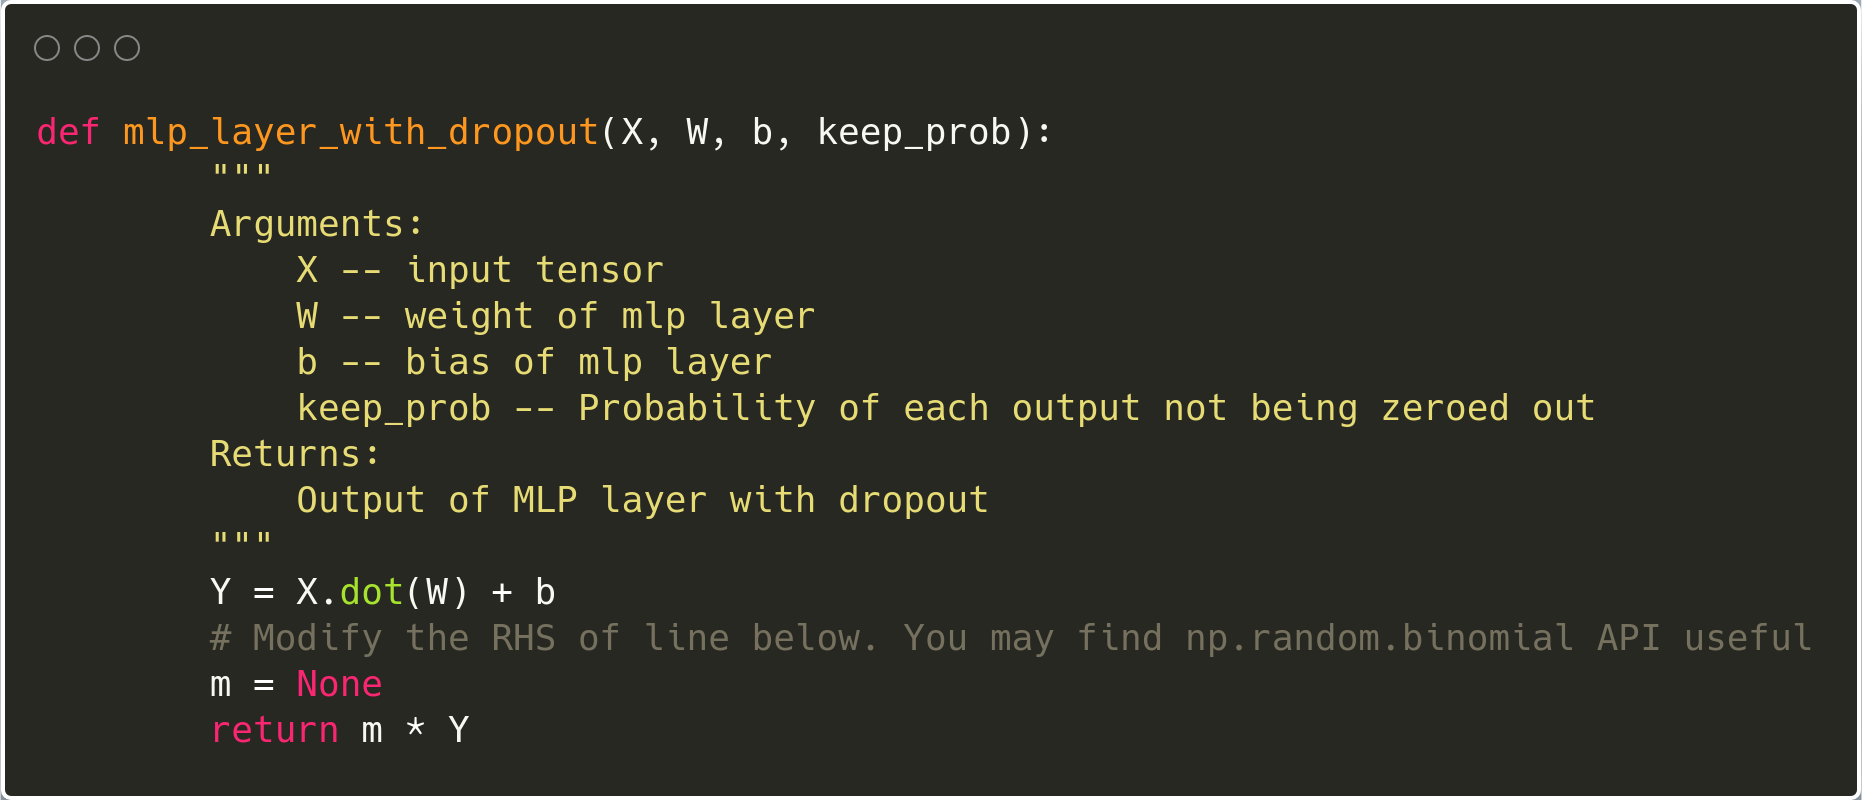
\includegraphics[width=0.9\textwidth]{images/quiz_4_4_3_1a.png}

Please write the line of code below the comment "Modify the RHS.."

You can check that your function is correct using the following test code:

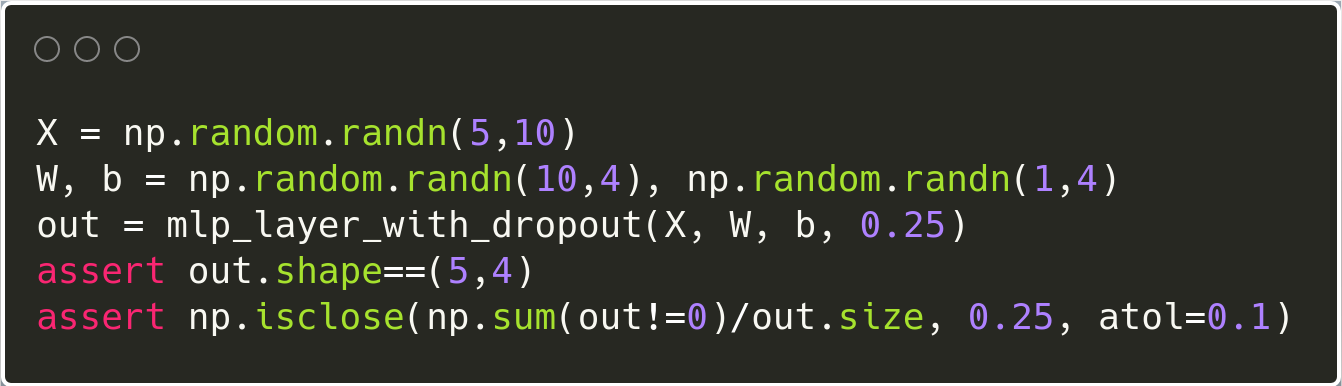
\includegraphics[width=0.7\textwidth]{images/quiz_4_4_3_1b.png}

% Desc Reference: https://numpy.org/doc/stable/reference/random/generated/numpy.random.binomial.html

% FIB

\end{frame}


\begin{frame}
\section{}
Consider the following implementation of a MLP layer with dropout in numpy:

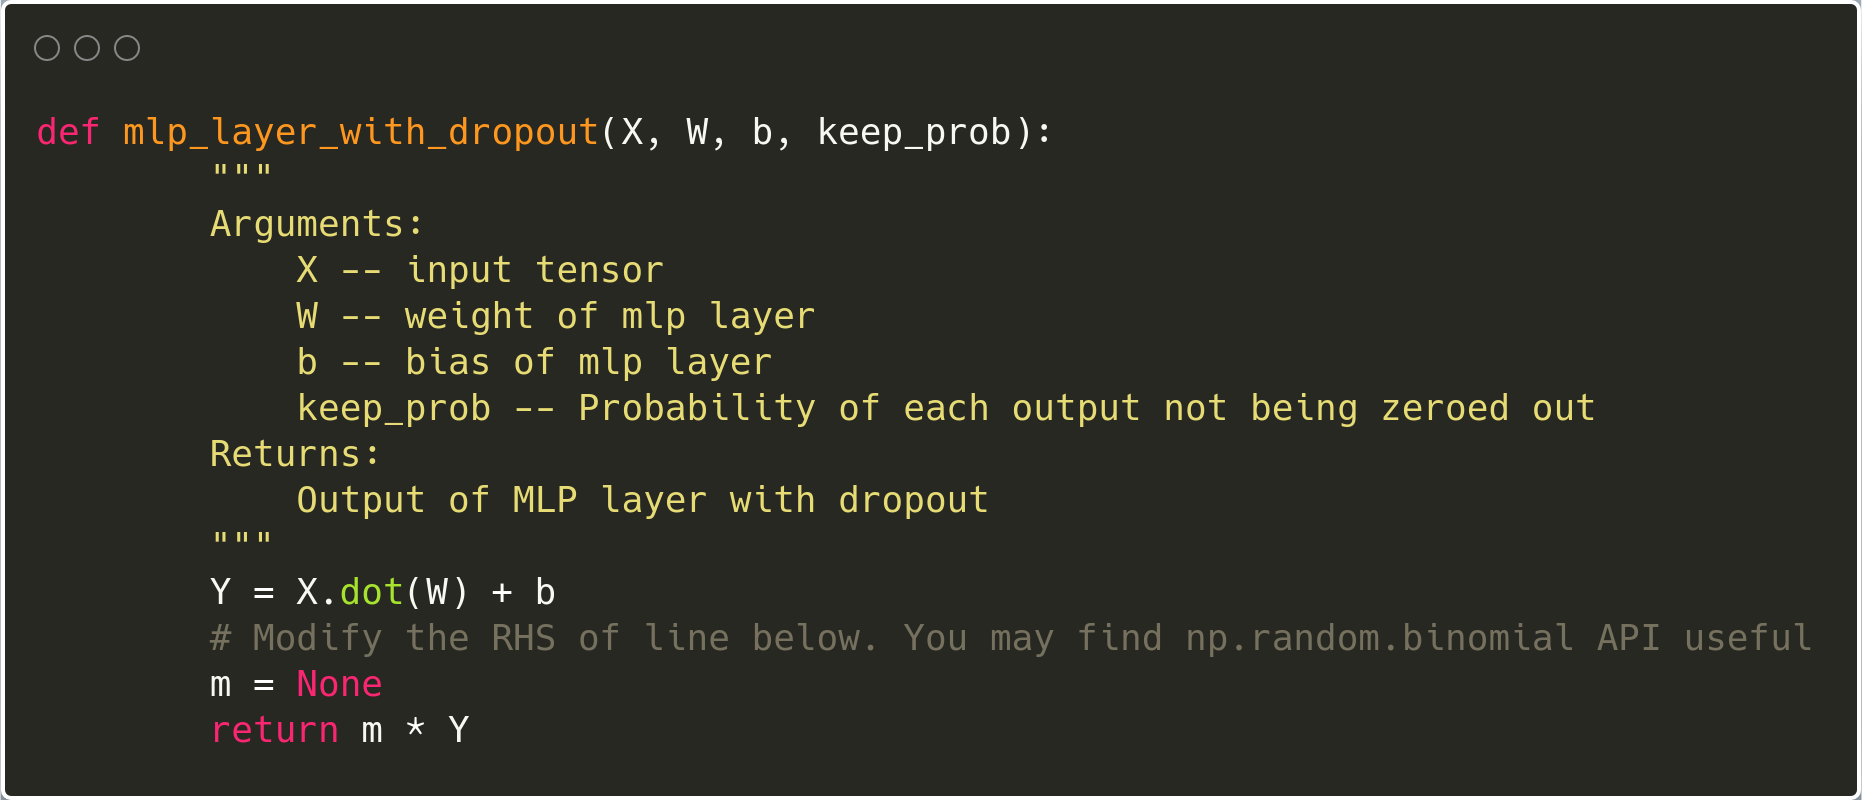
\includegraphics[width=0.9\textwidth]{images/quiz_4_4_3_2a.png}

Please write the line of code below the comment "Modify the RHS.."

You can check that your code is correct using the following test code:

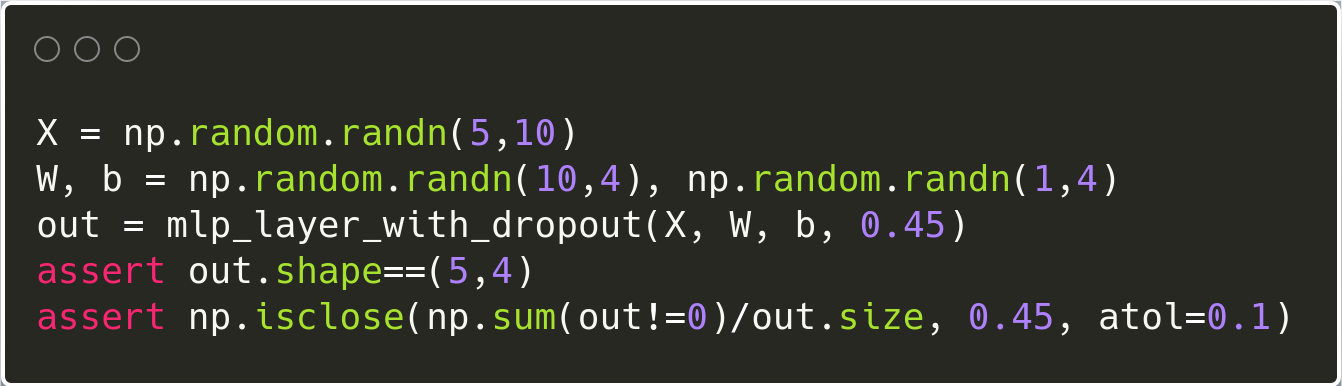
\includegraphics[width=0.7\textwidth]{images/quiz_4_4_3_2b.png}

% Desc Reference: https://numpy.org/doc/stable/reference/random/generated/numpy.random.binomial.html
% FIB

\end{frame}


\begin{frame}
\section{}
Consider the following implementation of a MLP layer with dropout in numpy:

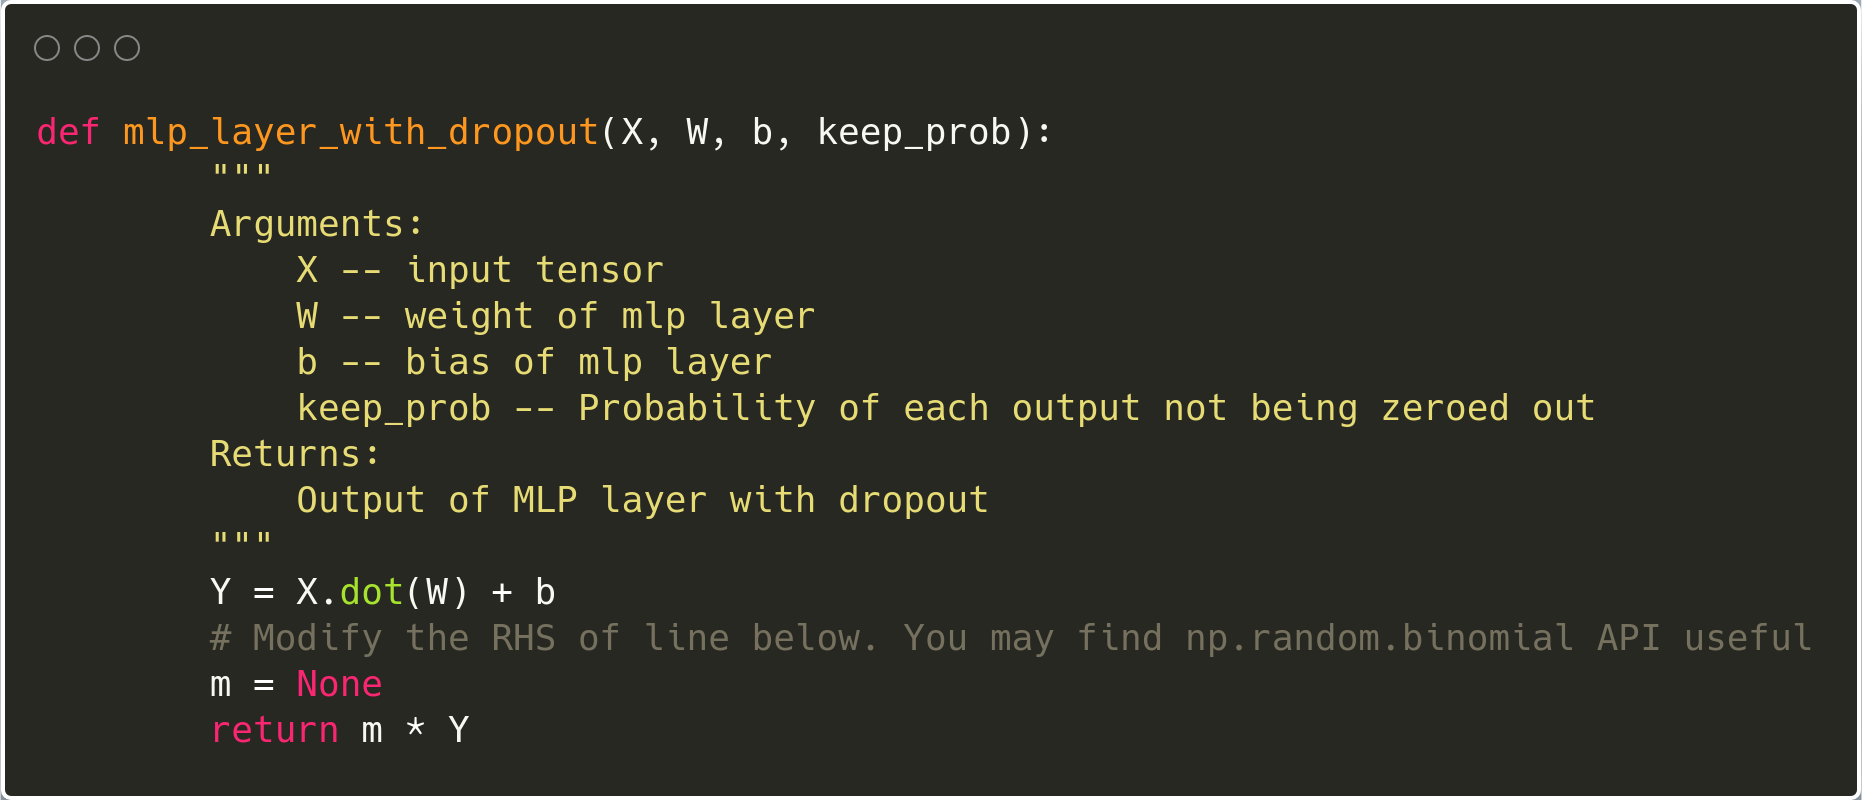
\includegraphics[width=0.9\textwidth]{images/quiz_4_4_3_3a.png}

Please write the line of code below the comment "Modify the RHS.."

You can check that your code is correct using the following test code:

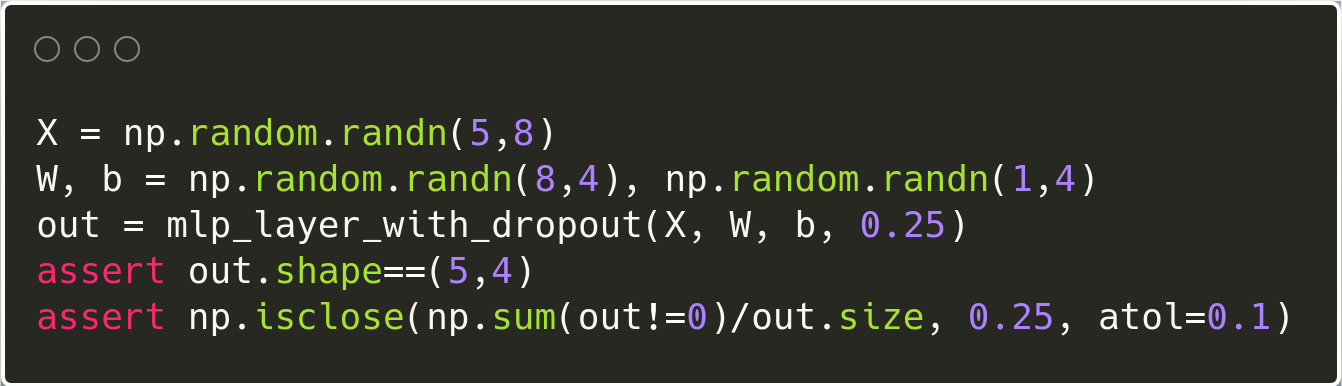
\includegraphics[width=0.7\textwidth]{images/quiz_4_4_3_3b.png}

% Desc Reference: https://numpy.org/doc/stable/reference/random/generated/numpy.random.binomial.html
% FIB

\end{frame}


\begin{frame}
\section{}
Consider the following implementation of a MLP layer with dropout in numpy:

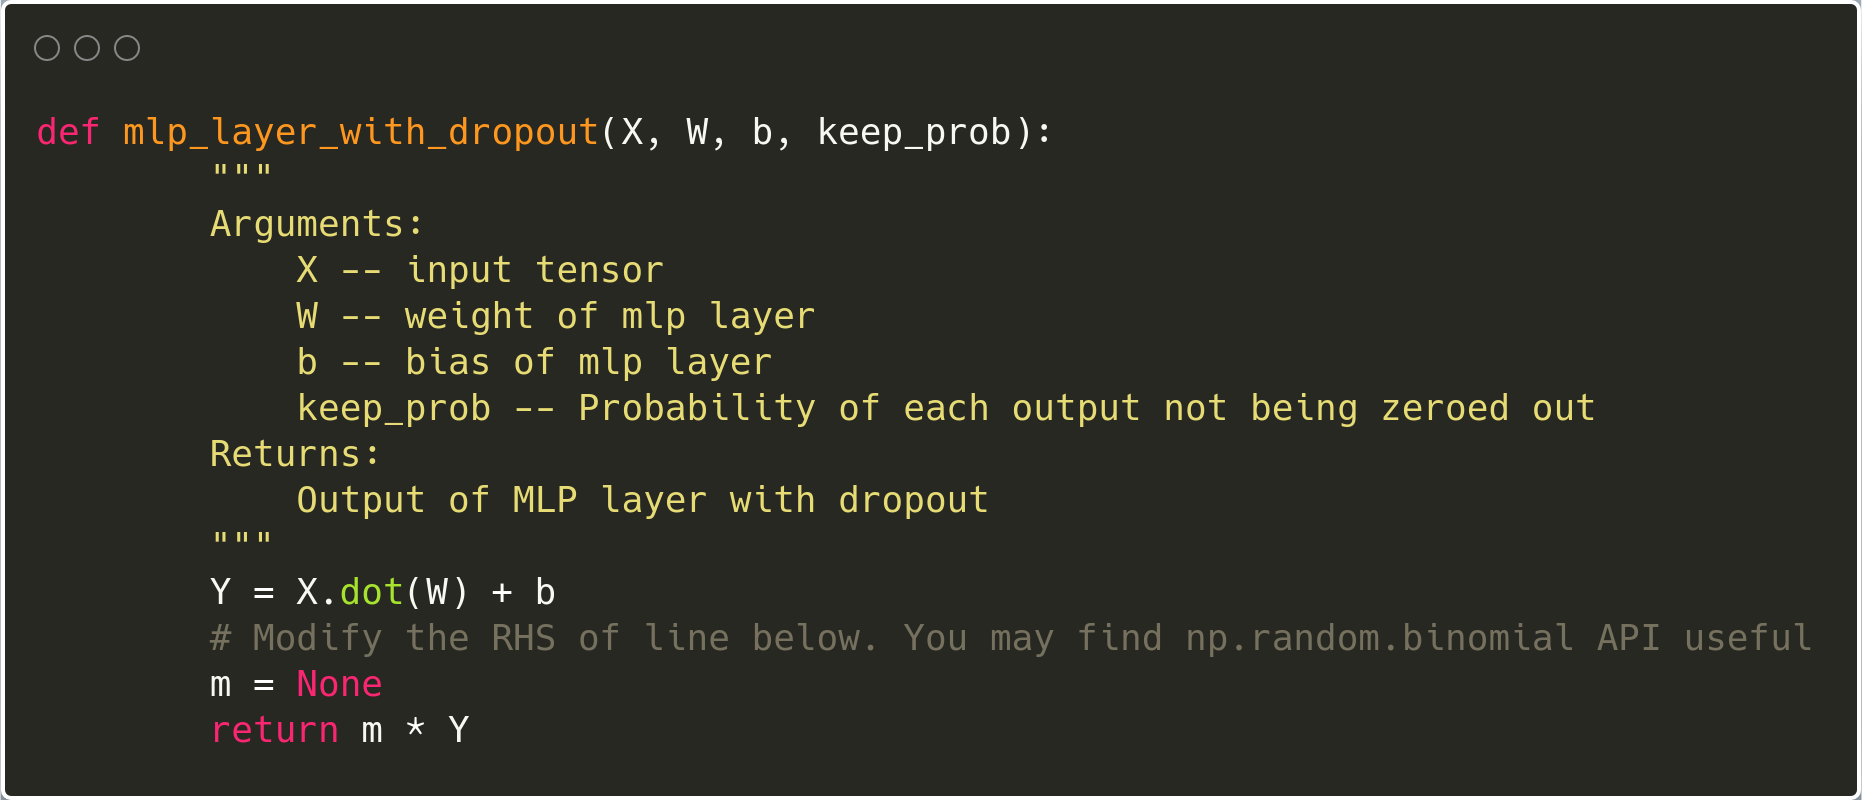
\includegraphics[width=0.9\textwidth]{images/quiz_4_4_3_4a.png}

Please write the line of code below the comment "Modify the RHS.."

You can check that your code is correct using the following test code:

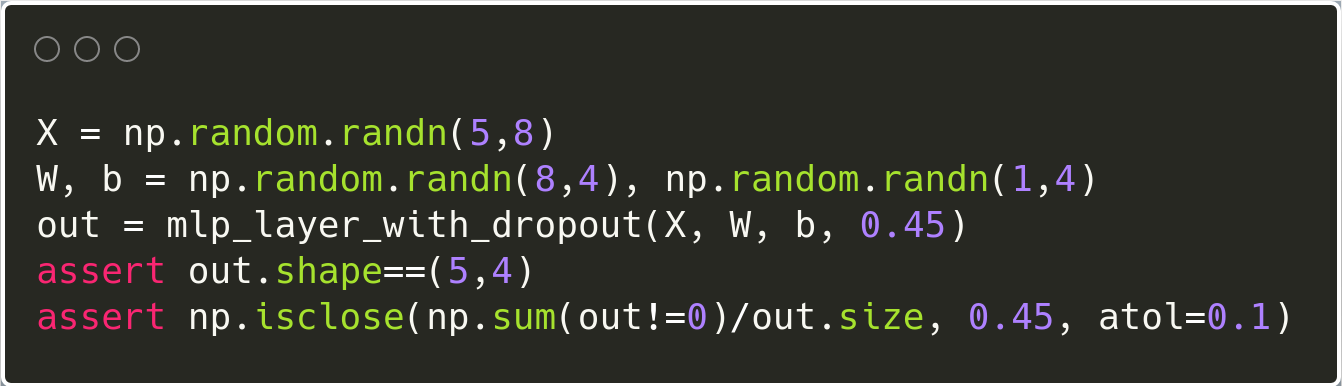
\includegraphics[width=0.7\textwidth]{images/quiz_4_4_3_4b.png}

% Desc Reference: https://numpy.org/doc/stable/reference/random/generated/numpy.random.binomial.html

% FIB

\end{frame}
